\section*{سوال ۱}

شبیه سازی یک مثال
\lr{(Real-Time Scheduling)}
در
\lr{True Time}
در نرم افزار متلب و ارایه یک گزارش (رجوع به اسلاید شماره دو)

\section*{جواب سوال ۱}

\begin{comment}
\begin{figure}[h]
	\centering
	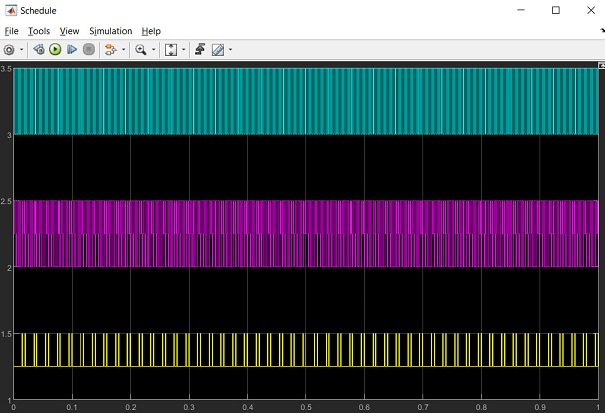
\includegraphics{6.jpg}
	\label{fig:label4}
\end{figure}
\end{comment}

\section*{گزارش کار با نرم‌افزار MATLAB و اجرای TrueTime}

در ابتدا، به دایرکتوری مورد نظر برای فعال‌سازی TrueTime در متلب مراجعه کردیم با این دستور:
\begin{figure}[h]
	\centering
	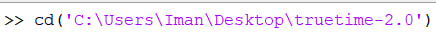
\includegraphics{12.jpg}
	\label{fig:label4}
\end{figure}


سپس، ماژول TrueTime با استفاده از دستور زیر فعال شده است:

\begin{figure}[h]
	\centering
	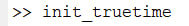
\includegraphics{13.jpg}
	\label{fig:label4}
\end{figure}

برای مشاهده محتوای دایرکتوری فعلی، از دستور \texttt{ls} استفاده شده است:

\begin{figure}[h]
	\centering
	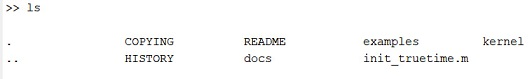
\includegraphics{14.jpg}
	\label{fig:label4}
\end{figure}

بعد از آن، به دایرکتوری \texttt{examples} و سپس به زیر دایرکتوری \texttt{threeservos} مراجعه شده است. در این قسمت، با کلیک روی فایل با فرمت slx ، شبیه‌سازی \texttt{threeservos} اجرا شده است.

\begin{figure}[H]
	\centering
	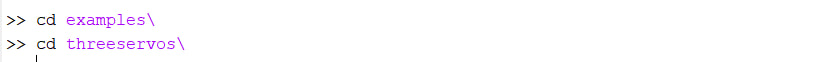
\includegraphics{15.jpg}
	\label{fig:label4}
\end{figure}

\newpage

\section*{بررسی فایل‌های داخل فولدر \lr{threeservos}}

با توجه به فایل‌های موجود در فولدر و فرمت‌ها و نام‌های موجود، فایل \texttt{threeservos.slx} فایل اصلی برنامه است. فایل‌های با پسوند \texttt{.slx} فایل‌های مدل‌سازی Simulink در MATLAB هستند و معمولاً برای شبیه‌سازی سیستم‌های کنترلی و دینامیکی استفاده می‌شوند.

فایل‌های دیگر با پسوند \texttt{.m} همگی اسکریپت‌ها یا توابع MATLAB هستند که توسط فایل \texttt{threeservos.slx} فراخوانی می‌شوند یا به تنهایی اجرا می‌شوند.

\begin{figure}[H]
	\centering
	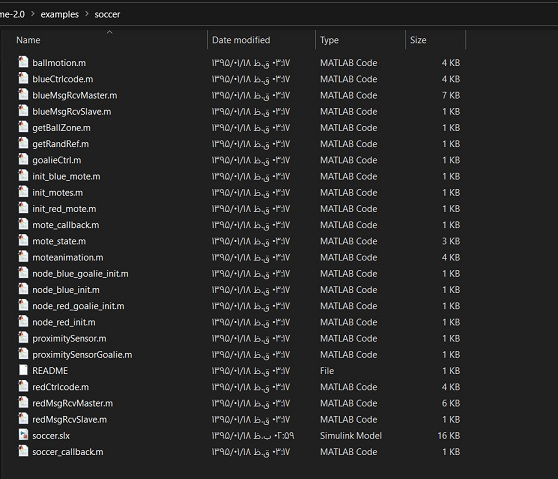
\includegraphics{2.jpg}
	\label{fig:label4}
\end{figure}

\newpage

\section*{محتویات فایل \lr{threeservos.slx}}

برای تشخیص دقیق‌تر، فایل \texttt{threeservos.slx} را در MATLAB باز کردیم و به محتوای آن نگاهی می‌اندازیم.

\begin{figure}[H]
	\centering
	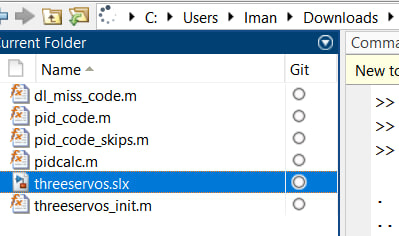
\includegraphics{4.jpg}
	\label{fig:label4}
\end{figure}

\begin{figure}[H]
	\centering
	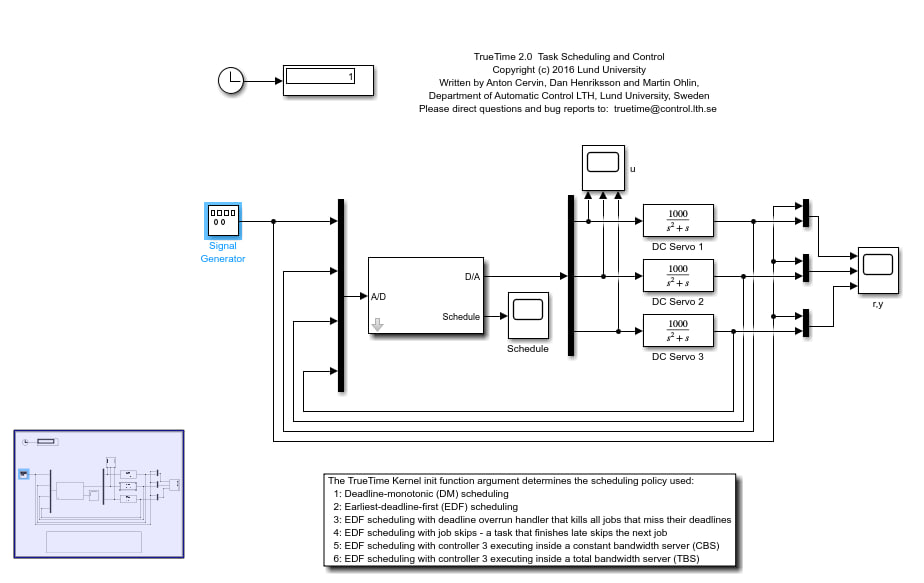
\includegraphics{17.jpg}
	\label{fig:label4}
\end{figure}

\newpage

\section*{تصاویر ران برنامه}

\begin{figure}[H]
	\centering
	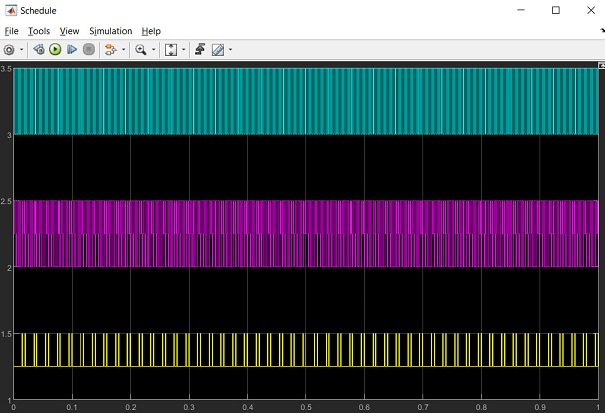
\includegraphics{6.jpg}
	\label{fig:label4}
\end{figure}

\begin{figure}[H]
	\centering
	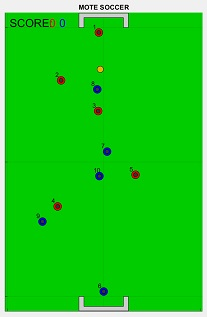
\includegraphics{7.jpg}
	\label{fig:label4}
\end{figure}

\begin{figure}[H]
	\centering
	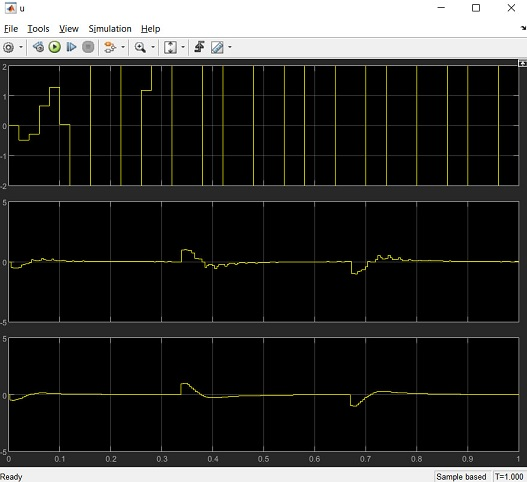
\includegraphics{8.jpg}
	\label{fig:label4}
\end{figure}

\begin{figure}[H]
	\centering
	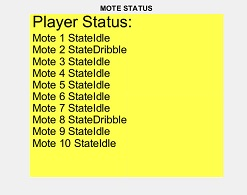
\includegraphics{9.jpg}
	\label{fig:label4}
\end{figure}

\begin{figure}[H]
	\centering
	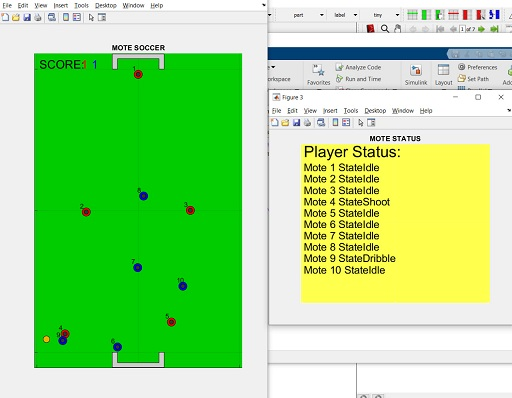
\includegraphics{10.jpg}
	\label{fig:label4}
\end{figure}

\newpage

\section*{کد \lr{soccer_callback.m}}

تابع فراخواننده‌ی این شبیه‌سازی در برنامه‌ی متلب:

\begin{figure}[H]
	\centering
	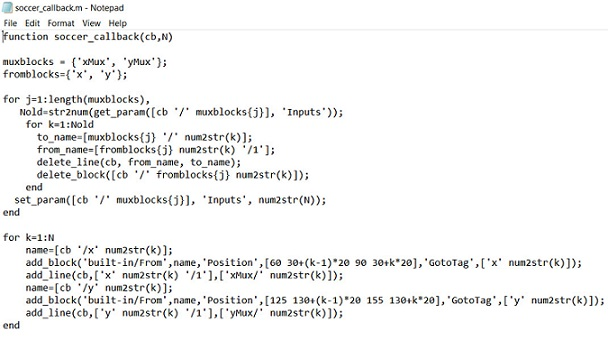
\includegraphics{16.jpg}
	\label{fig:label4}
\end{figure}

\newpage

\section*{روند ران کردن برنامه}

فولدر
\lr{truetime2}
را دریافت می‌کنیم و با اجرای دستور
\lr{init_truetime}
و سپس وارد این فولدر شدن با دستور
\lr{init_motos}
و سپس با دستور
\lr{soccer}
برنامه ران می‌شود.

\section*{توضیح کد}

\begin{enumerate}
	\item \textbf{تعریف تابع:} تابعی با نام \texttt{soccer\_callback} با دو ورودی، \texttt{cb} و \texttt{N}، تعریف شده است.
	\item \textbf{تعریف متغیر‌ها:} دو آرایه از رشته‌ها تعریف شده‌اند؛ یکی برای بلوک‌های \texttt{Mux} و دیگری برای بلوک‌های \texttt{From}.
	\item \textbf{حلقه اول:} این حلقه برای هر یک از بلوک‌های \texttt{Mux} اجرا می‌شود:
	\begin{itemize}
		\item تعداد ورودی‌های فعلی بلوک \texttt{Mux} بازیابی می‌شود.
		\item یک حلقه داخلی برای هر ورودی بلوک \texttt{Mux} اجرا می‌شود و:
		\begin{itemize}
			\item اتصالات موجود بین بلوک‌های \texttt{From} و \texttt{Mux} حذف می‌شوند.
			\item بلوک‌های \texttt{From} موجود حذف می‌شوند.
		\end{itemize}
		\item تعداد ورودی‌های بلوک \texttt{Mux} به مقدار جدید \texttt{N} تنظیم می‌شود.
	\end{itemize}
	\item \textbf{حلقه دوم:} این حلقه برای ایجاد بلوک‌های جدید از نوع \texttt{From} و اتصال آن‌ها به بلوک‌های \texttt{Mux} اجرا می‌شود.
\end{enumerate}

برنامه به اتمام می‌رسد پس از اجرای دو حلقه‌ی \texttt{for} که در آنها، تمامی بلوک‌های مرتبط حذف شده و بلوک‌های جدید اضافه می‌شوند. پس از اجرای کامل دومین حلقه، تابع به پایان خواهد رسید.


\newpage

\section*{آموزش نصب و فعال‌سازی MATLAB ورژن \lr{2023a}}

\begin{enumerate}
	\item قبل از شروع نصب، اتصال به اینترنت را قطع می‌کنیم.
	\item فایل مورد نظر از حالت فشرده خارج شده است.
	\item فایل \lr{R2023a\_Windows.iso} را با استفاده از یک برنامه‌ی درایو مجازی Mount نموده و نصب را شروع می‌کنیم.
	\item فایل \texttt{Setup} را اجرا کرده و در قسمت \lr{Enter File Installation Key}، سریال گفته شده را وارد کردیم:
	
	\item در مرحله \lr{Select License File}، فایل \texttt{license.lic} واقع در پوشه‌ی \texttt{Crack} را انتخاب می‌کنیم.
	\item پس از نصب، نرم‌افزار را اجرا نمی‌کنیم.
	\item فایل \texttt{libmwlmgrimpl.dll} را از پوشه‌ی \texttt{Crack} به مسیر گفته شده کپی کردیم و فایل را در آن مسیر جایگزین می‌نماییم.
	کپی کرده و فایل موجود در آن مسیر را جایگزین می‌کنیم.
	\item حال می‌توانید نرم‌افزار را اجرا کنیم.
	\item در صورت نیاز به آپدیت، فایل آپدیت با فرمت \texttt{iso} را مانت کرده و فایل \texttt{Update.cmd} را اجرا می‌کنیم.
	\item مجدداً فایل \texttt{libmwlmgrimpl.dll} را جایگزین می‌کنیم.
\end{enumerate}
